\documentclass{bioinfo}
\copyrightyear{2012}
\pubyear{2012}

\begin{document}
\firstpage{1}

\title[Pathway-based visualization of cross-platform microarray datasets]{Pathway-based visualization of cross-platform microarray datasets}
\author[Clemens Wrzodek \textit{et~al}]{Clemens Wrzodek\,$^{1\footnote{to whom correspondence should be addressed}}$, Johannes Eichner\,$^{1}$ and Andreas Zell\,$^1$}

\address{$^{1}$Center for Bioinformatics Tuebingen (ZBIT), \\University of Tuebingen, 72076 T\"ubingen, Germany}
\history{Received on XXXXX; revised on XXXXX; accepted on XXXXX}

\editor{Associate Editor: XXXXXXX}

\maketitle

\begin{abstract}

\section{Motivation:}
Text Text Text  Text Text Text Text Text Text Text Text
Text  Text Text Text Text Text Text Text Text Text  Text Text Text Text Text Text Text Text Text  Text Text Text Text Text Text Text Text Text  Text Text Text Text Text Text Text Text Text  Text Text Text Text Text Text Text Text Text  Text Text Text Text Text.

\section{Results:}
Text  Text Text Text Text Text Text Text Text Text  Text Text Text Text Text Text Text Text Text  Text Text Text Text Text Text Text Text Text  Text Text Text Text Text Text

%\section{Availability:}

\section{Contact:} \href{clemens.wrzodek@uni-tuebingen.de}{clemens.wrzodek@uni-tuebingen.de}
\end{abstract}

\section{Introduction}

During the first years after the invention of microarrays, researchers focused their experiments largely on messenger RNA (mRNA) expression data. Therefore, many analysis and visualization methods have been developed especially for mRNA datasets. Until today, multiple different microarray platforms have been developed. These different platforms include, for example, microarrays to measure the expression of micro RNAs (miRNAs), proteins, or even the amount of DNA methylation in defined genomic regions \citep{Hoheisel2006}. For all of those platforms, preprocessing, analysis and visualization methods also became available. But, until today, methods that can integratively visualize multiple microarray datasets, coming from multiple different platforms are very rare.

We introduce a method, for integrated pathway-based visualization of multiple different microarray datasets. 

% Warum ist PW-basierte visualisierung, grade f�r mehrere Datentypen, besser als UCSC genome browser oder anderes.

Microarrays are probe-based and these probes are mostly not spread randomly across the genome. Probes are usually picked for interesting genes or regions, which includes genes, that are important for certain pathways. Region-based visualization methods, like the USCS Genome Browser \citep[see][]{UCSCBrowser}, may be suitable for visualization if researchers already know some regions of interest. But in general, they are not good visualization methods for probe-based datasets.

To get a starting point for microarray analysis and because microarrays usually contain probes for most important pathways, the popular pathway enrichment analysis is very often performed on microarray datasets. And this is already the ending point of most pathway analysis methods. Some applications offer users to show the pathway enrichments as bar plots, but visualizing the pathways and plotting the microarray data directly in the pathway are rare features. For these reasons, we show how to integratively visualize data from multiple different microarray datasets in a pathway.

% TODO: Erw�hnen dass mRNA knoten einf�rbung ein "alter hut ist", aber das besodere bei den anderen 3 datentypen ist.


We present a novel method that includes visualizing pathways and changing the pathway to reflect expression data from mRNA, miRNA, DNA methylation and (phospho-) protein datasets.


% The amount of available expression datasets is growing rapidly from day to day. But not only the

There are other tools, specialized in pathway analysis (e.g., Ingenuity, ), or in pathway visualization (Cytoscape, KEGG Atlas). Some even offer visualizing data in a pathway (GenMAPP, KEGG Array, Symony programm). 

TODO: das h�chste der gef�hle sind methoden um 2 farben in 1 knoten, aber keiner kann DNA methylation oder sogar miRNA knoten rein.

TODO Johannes: Kannst du 1-2 S�tze jeweils zu Cytoscape, Ingenuity, eventuell noch Cytoscape + Plugins schreiben?


Related Work. Abgrenzung zu GenMAPP und Ingenuity, Cytoscape, KEGG Atlas, KEGG Array; Siehe auch Kohlbacher-Nils Paper, S. Symons paper (niselt).
Gibt es ueberhaupt ein Tool, welches alle 4 Datentypen (miRNA, etc) visualisieren kann?


No method today for high-dimensional, heterogeneous cross-platform datasets.

%\begin{methods}
\section{Methods}

This method starts by translating KGML documents from the KEGG PATHWAY database to GraphML documents. Optionally, one can create an overlay graph that shows the original KEGG pathway picture in the background to reduce the lack of information that occurs by limitations of the KGML format. Afterwards, the nodes are modified to reflect mRNA expression, protein expression and DNA methylation changes. As a last step, nodes are being added for miRNAs and miRNA expression data is visualized in the pathway. See Figure~\ref{fig:visualization_steps} for a graphical description of all those visualization steps.

%Please note that the described procedures are only valid for processed microarray datasets with ``observations". In this context, observations can be any statistical significance or comparative measure (we used \emph{p}-values or fold-changes).

\subsection{Pathway visualization}

The basic prerequisite for pathway-based visualization is visualizing the pathway itself. We are using KEGGtranslator \citep[see][]{Wrzodek2011} to perform a basic conversion of the KEGG KGML documents to GraphML and to annotate all nodes with entrez gene identifiers. In short, KEGGtranslator converts all KGML entries to nodes and all relations to edges. Some basic errors are corrected automatically and appropriate shapes, colors and labels are inferred. Then, all nodes are annotated with various identifiers and further information. The resulting document is the base for our visualizations. At this point, it is important to note that KEGG usually draws referenced pathways as rectangular nodes with rounded corners, small molecules as circles, and single gene products (e.g., enzymes) as well as gene families as rectangles. This means that one rectangular node can consist of multiple different enzymes, depending on the KEGG definition.

\subsection{Visualization of messenger RNA expression data}

Visualization of mRNA datasets is straightforward by somehow gene-centering the input data and then changing the node color according to this value. As input, this method requires processed mRNA datasets with gene identifiers and ``observations". In this context, ``observations" can be any statistical significance or comparative measure (we used \emph{p}-values or fold-changes). Then, for each node in the pathway, one value must be calculated. Therefore, all probes that belong to a node are gathered from the input dataset and then the mean or median is calculated. Another possibility is to take the most important probe (i.e., $\min\emph{p}-value$ or $\max|fold-change|$) to get a single value for each pathway node.
This value is then used to calculate a color for the node. For fold-changes (which are usually $log_2$ values), we color every node with a fold-change $\geq2$ red and all fold-changes $\leq-2$ blue. Fold-changes of zero are defined to have a white color and colors between $\pm2$ are faded from blue or red to white, depending on the actual fold-change. The same procedure can be used for \emph{p}-values, except that just one minimum threshold and one minimum color must be defined. Furthermore, the color for \emph{p}-values should not be changed on a linear, but on a log-scale. See Figure~\ref{fig:visualization_steps}c) for an example of visualized mRNA data.


\subsection{Visualization of protein and protein modification expression data}

Visualization of protein datasets is performed by adding small boxes below pathway nodes and changing the color of the boxes according to the corresponding protein expression data. Protein datasets usually have identifiers, like Entrez Gene IDs, UniProt IDs, etc. which allows to make a straightforward mapping to pathway nodes. Then, all values must be collected and a color must be calculated for each node in the same way as already described for mRNA datasets.

Protein modification datasets must be treated differently. They usually not only contain one expression values for the basic form of the protein, but also for some phosphorylated or likewise modified form. Therefore, separate boxes are created below each pathway node for all modifications. These boxes are labeled according to the modification. Furthermore, the color for each box must only be calculated on probes that match the pathway node and the modification of each box.


\subsection{Visualization of DNA methylation data}

Ein Wert nur als Hinweis, hier geht etwas [click gibt details?]. fold-change wird zu box von -2 bis +2, p-value im grunde ein bar-blot von 1 bis 0.00005 oder so...

Einzelner Wert mit binning und $\frac{\sum\limits_{i=1}^n\log_2 x}{n}$, f�r fold-changes oder so peak detection m�glich und max. peak anzeigen.

\textbf{Johannes.}


\subsection{Visualization of micro RNA expression data}
erst auf Targets eingehen.

Dann wie targets in graph gef�gt werden

Dann wie knoten eingef�rbt werden.


\subsection{OFFENE FRAGEN}
Sollten wir hier einfaerbung nach enrichment p-values bzw. den "metabolic pathways"-pathway erwaehnen? Oder lieber fuer spaetere publikationen "aufspaaren"?

%\end{methods}



\section{Results and discussion}

Gesamtkonzept und Ergebnisse / Bilder vorstellen

hier erw�hnen, dass methoden in InCroMAP drin sind? oder lieber in conslutions?






\begin{figure*}[t]
\centering
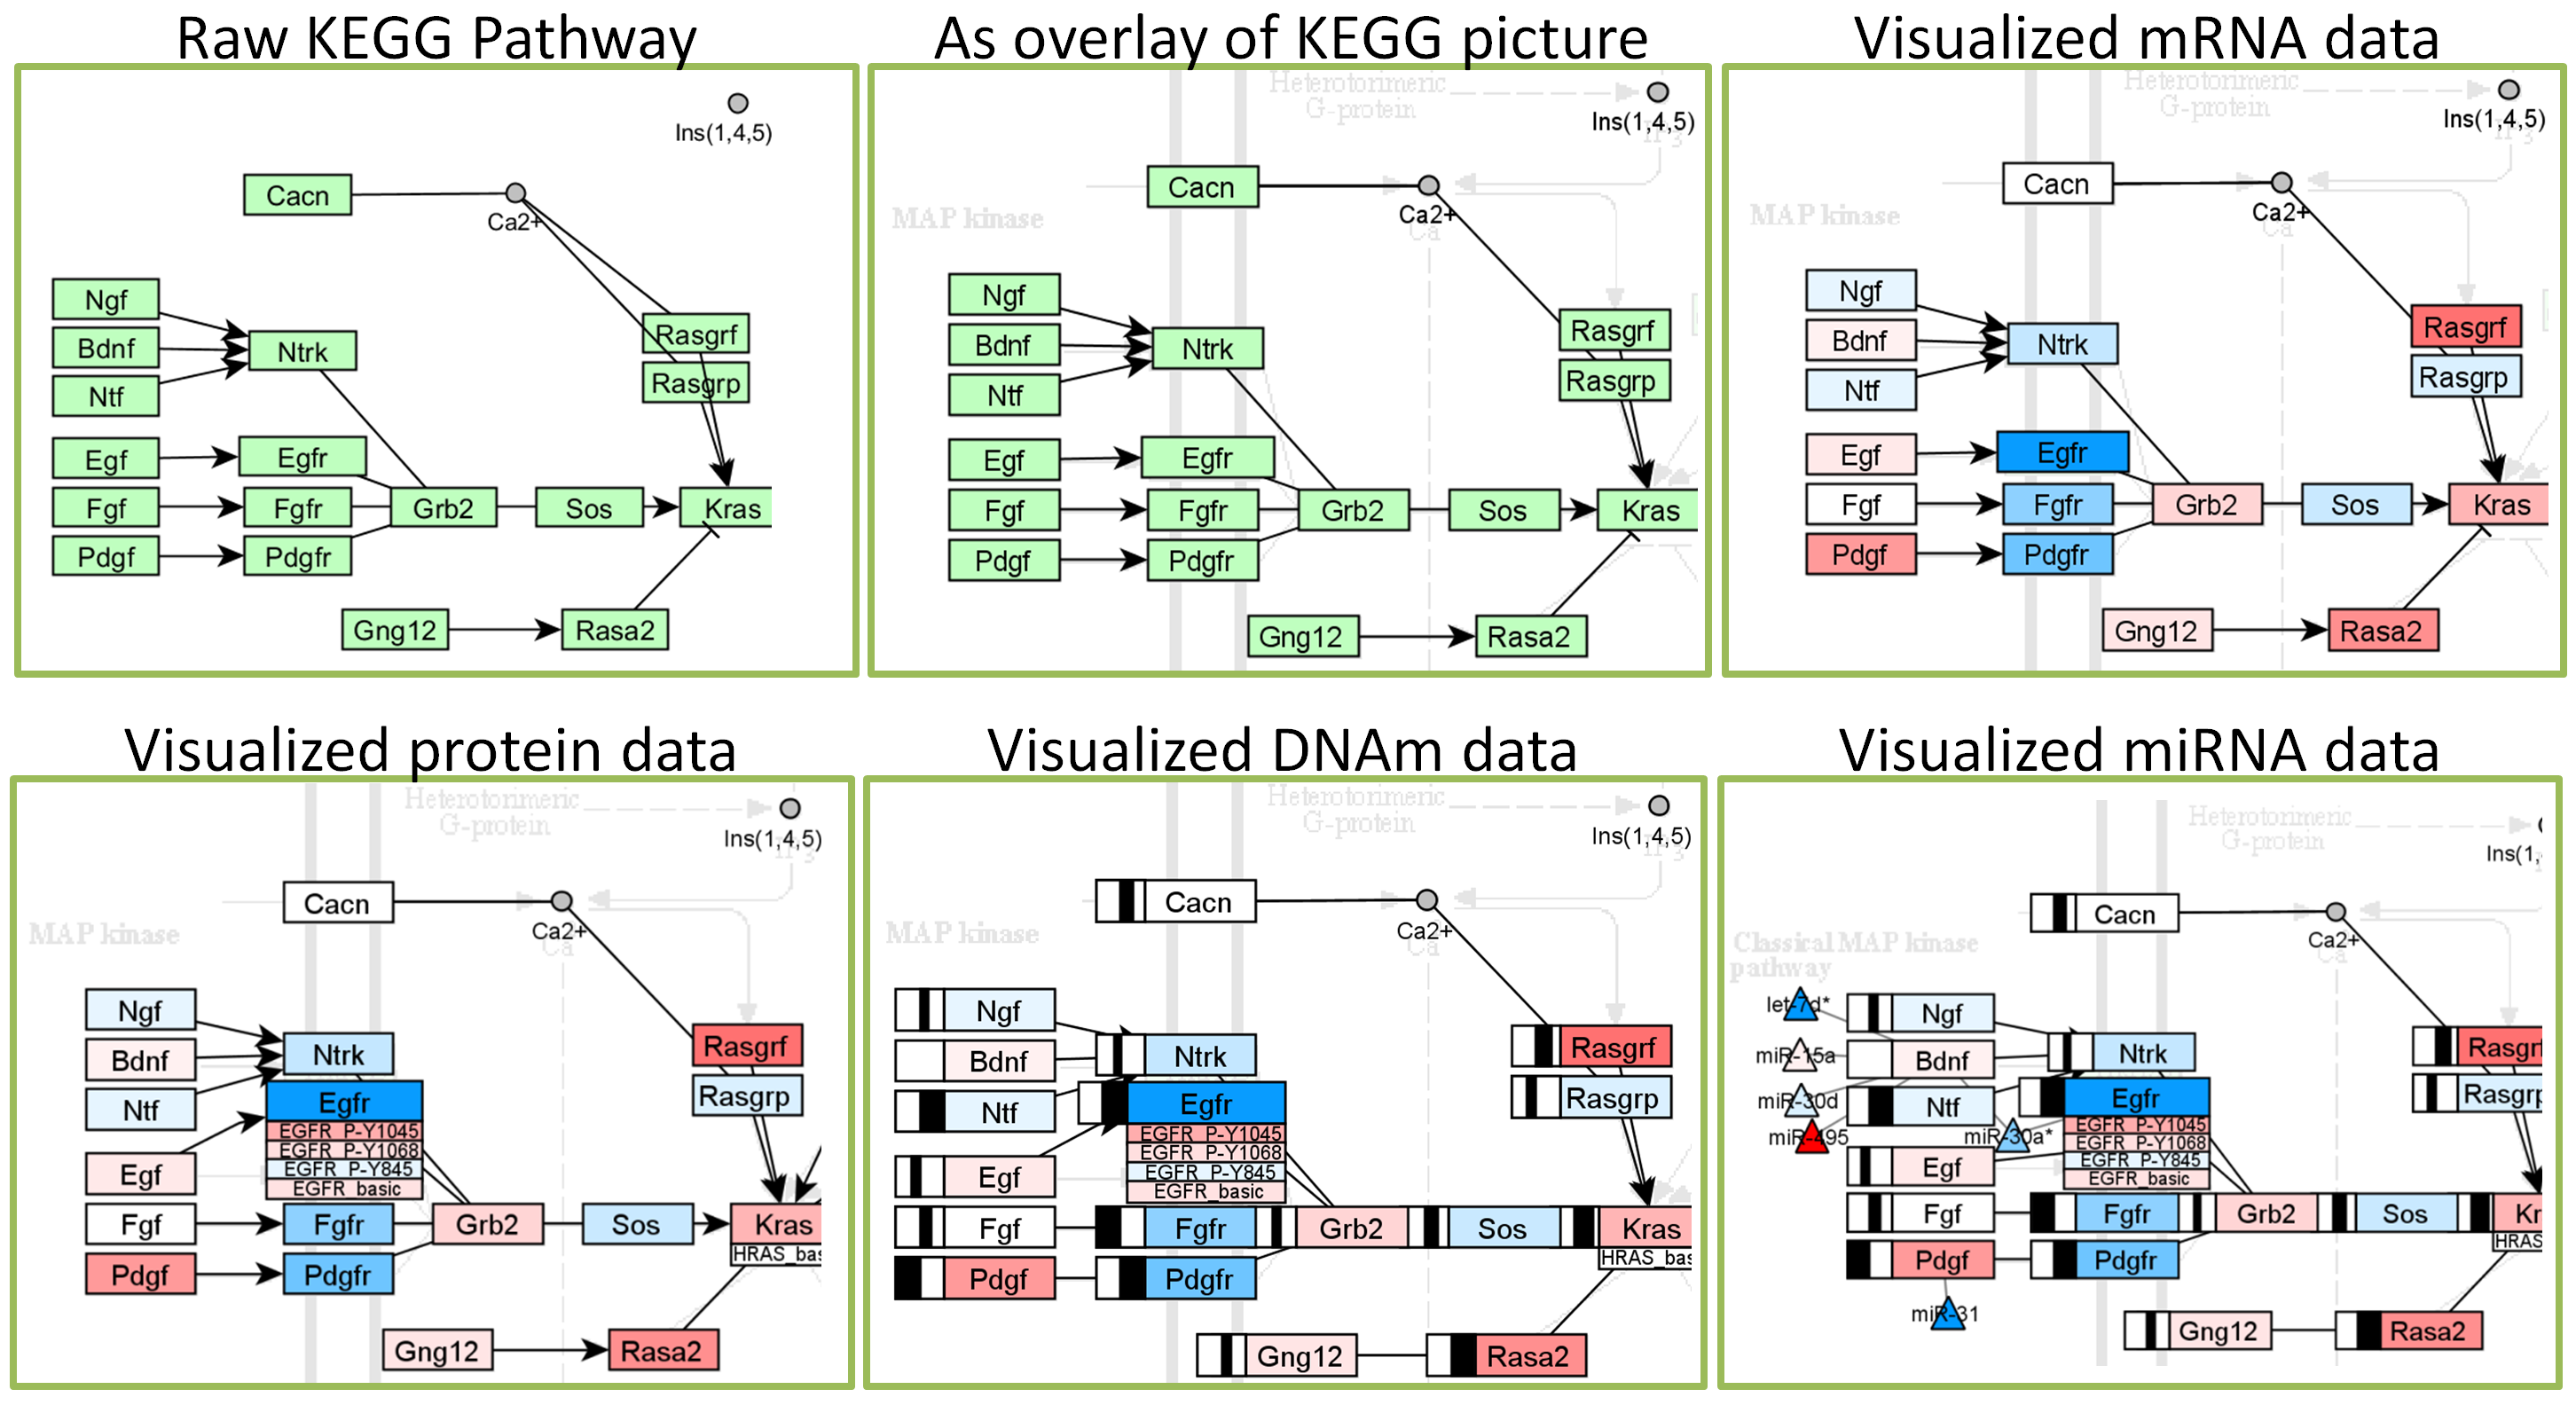
\includegraphics[width=1.0\textwidth]{figures/visualization-steps.PNG}
\caption{MAPK signaling pathway.}\label{fig:visualization_steps}
\end{figure*}



\section{Conclusion}

TODO



\section*{Acknowledgement}
We gratefully acknowledge contributions from Andreas Dr\"ager and Finja B\"uchel, as well as the whole MACRCAR consortium.

\paragraph{Funding\textcolon} The research leading to these results has received funding from the Innovative Medicine Initiative Joint Undertaking (IMI JU) under grant agreement nr. 115001 (MARCAR project).

\bibliographystyle{natbib}
%\bibliographystyle{achemnat}
%\bibliographystyle{plainnat}
%\bibliographystyle{abbrv}
%\bibliographystyle{bioinformatics}
%\bibliographystyle{plain}

\bibliography{document}
%TODO: When paper is ready, comment \bibliography line and add content of document.bbl here.

\end{document}
